\documentclass[11pt,a4paper]{article}

\usepackage{tikz}
\usepgflibrary{offsetpath}

\begin{document}

\section{Testing the pgf library \texttt{offsetpath} only}

\subsection{Using \textbackslash pgfoffsetpath}
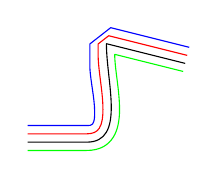
\begin{tikzpicture}[line join=bevel]
  \path[save path=\savedpath] (0,0) -- (.75,0) to[out=0, in=-90] (1,1.25) -- (2,1);
  \pgfoffsetpath{\savedpath}{0pt}
  \color{black}
  \pgfusepathqstroke
  \pgfoffsetpath{\savedpath}{3pt}
  \color{red}
  \pgfusepathqstroke
  \pgfoffsetpath{\savedpath}{6pt}
  \color{blue}
  \pgfusepathqstroke
  \pgfoffsetpath{\savedpath}{-3pt}
  \color{green}
  \pgfusepathqstroke
\end{tikzpicture}\newline
Note the uneven spacing at the upper join.

\subsection{Using methods that scale correctly}
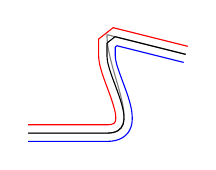
\begin{tikzpicture}[line join=bevel]
  \path[draw=gray, save path=\savedpath] (0,0) -- (1,0) to[out=0, in=-90] (1,1.25) -- (2,1);
  % Note how the path offset by 0 differs from the original path
  \pgfoffsetpathfraction{\savedpath}{6pt}{0}
  \color{black}
  \pgfusepathqstroke
  \pgfoffsetpathqfraction{\savedpath}{6pt}{.5}
  \color{red}
  \pgfusepathqstroke
  \pgfoffsetpathindex{\savedpath}{6pt}{2}{5}
  \color{blue}
  \pgfusepathqstroke
\end{tikzpicture}\newline
The gray line is the original path. Note how it differs from the black path (offset=0).

\section{Testing the pgf (not TikZ) library \texttt{nfold}}

\usepgflibrary{nfold}

\begin{pgfpicture}
  \pgfpathmoveto{\pgfpoint{0}{0}}
  \pgfpathlineto{\pgfpoint{5cm}{0}}
  \pgfsetlinewidth{10pt}
  \pgfsetinnerlinewidth{9pt}
  \pgfsetarrows{<->}
%  \pgfusepath{stroke}
  \pgfusepath{stroke,/pgf/nfold=4}
\end{pgfpicture}
\vspace{10pt}\newline
The wide arrow tips are expected; this is because \verb|arrows.meta| is not loaded.

\subsection{Support for pgf rectangles}
Note that this is \emph{not} called by TikZ' \texttt{rectangle} option.

\begin{pgfpicture}
  \pgfpathmoveto{\pgfpoint{-1cm}{-1cm}}
  \pgfpathlineto{\pgfpoint{1cm}{-1cm}}
  \pgfpathrectangle{\pgfpointorigin}{\pgfpoint{20pt}{20pt}}
  \pgfpathlineto{\pgfpoint{-1cm}{0cm}}
  \pgfsetlinewidth{3pt}
  \pgfsetinnerlinewidth{2pt}
  \pgfusepath{stroke,nfold}
\end{pgfpicture}

\subsection{A path without a moveto (slight bug at the moment)}
Compare
\begin{pgfpicture}
  \pgfpathlineto{\pgfpoint{1cm}{1cm}}
  \pgfpathlineto{\pgfpoint{2cm}{0cm}}
  \pgfsetlinewidth{3pt}
  \pgfsetinnerlinewidth{2pt}
  \pgfusepath{stroke}
\end{pgfpicture}
to
\begin{pgfpicture}
  \pgfpathlineto{\pgfpoint{1cm}{1cm}}
  \pgfpathlineto{\pgfpoint{2cm}{0cm}}
  \pgfsetlinewidth{3pt}
  \pgfsetinnerlinewidth{2pt}
  \pgfusepath{stroke,nfold}
\end{pgfpicture}

\subsection{An example where \textbackslash pgf@prepare@start@of@path is not called}
Here the nfold preparation code must be injected into \verb|\pgf@path@check@proper|.
{
\makeatletter
\def\pgf@prepare@start@of@path{\pgferror{not called}}
\makeatother
\begin{pgfpicture}
  \pgfpathmoveto{\pgfpointorigin}
  \pgfpathlineto{\pgfpoint{1cm}{0cm}}
  % make the path non-proper by adding a dead moveto
  \pgfpathmoveto{\pgfpointorigin}
  \pgfsetlinewidth{.3cm}
  \pgfsetinnerlinewidth{.25cm}
  \pgfsetarrows{<->}
  \pgfusepath{stroke,tips/proper,nfold=3} % likely means "only draw tips on proper arrows"
\end{pgfpicture}
}

\end{document}
